\chapter{Machine Learning}

\section{Introduzione}

Il machine learning (ML) è un ramo dell'intelligenza artificiale che si concentra sullo sviluppo di sistemi in grado di migliorare le proprie prestazioni nell'esecuzione di un compito specifico attraverso l'apprendimento dall'esperienza, senza la necessità di una programmazione esplicita.
\textcite{mitchell1997ml} ne fornisce una definizione più formale:

\blockquote{A computer program is said to learn from experience $E$ with respect to some class of tasks $T$ and performance measure $P$ if its performance at tasks in $T$, as measured by $P$, improves with experience $E$.}

L'obiettivo in ambito ML è quello di sviluppare \textit{algoritmi di apprendimento} che producano \textit{modelli} a partire dai dati \parencite{zhou2021ml}, i quali costituiscono l'esperienza a cui si fa riferimento nelle definizioni presentate. Nel Paragrafo \ref{par:tassonomia} definiamo con precisione cosa intendiamo con ``modello" e ``algoritmo di apprendimento".

I dati non sono altro che istanze del dato problema che sono già state affrontate, e dalle quali, tramite un processo induttivo, si può ricavare un meccanismo col quale affrontarne altre mai incontrate. Questo processo è analogo al nostro apprendimento induttivo, in cui, a partire da esperienze pregresse, siamo in grado di formulare regole generali per affrontare situazioni nuove.
Non è un caso che modelli di ML come le reti neurali traggano forte ispirazione dall'anatomia e dalla fisiologia del cervello umano.

Per via della natura induttiva del processo di apprendimento, le risposte che si ottengono dai modelli di ML non possono essere certamente corrette in ogni caso, ma rappresentano stime basate sui dati a disposizione, soggette a un margine di errore che dipende dalla qualità e dalla quantità degli stessi.

Vi sono però due casi, presentati di seguito, in cui accontentarsi di una risposta probabilmente corretta, al posto di una la cui correttezza è dimostrabile logicamente, è preferibile, se non essenziale.
\begin{itemize}
    \item Problemi per cui non siamo in grado di formulare un algoritmo risolutivo basato su regole esplicite, anche perché può non esistere. Rientrano in questa categoria i problemi di riconoscimento del volto, di traduzione da una lingua a un'altra o di diagnosi medica basata su radiografie e risonanze magnetiche.
    
    \item Problemi per cui formulare una soluzione esplicita è possibile, se non facile, ma che sono proibitivi dal punto di vista computazionale. Nell'ambito dell'ottimizzazione combinatoria, ad esempio, l'adozione di modelli di ML si rivela vantaggiosa per la risoluzione di diversi problemi (\cite{bengio2021optim}).
\end{itemize}

In entrambi i casi, adottiamo un modello di ML con l'auspicio che le sue risposte si avvicinino il più possibile a quelle corrette, qualora il problema le ammetta. Tuttavia, l'approccio basato sul ML non è infallibile; non vi è alcuna garanzia che si riesca sempre a ottenere un siffatto modello.
    
\section{ML: Definizioni Preliminari}
\label{par:tassonomia}

Per evitare qualsiasi tipo di ambiguità, definiamo i termini e i concetti fondamentali in ambito ML di cui ci serviremo.

\begin{description}
    \item[Algoritmo di apprendimento (o di addestramento).] È una funzione 
    \begin{equation}
        l:(m, D) \rightarrow m'
    \end{equation}
    che allena il modello $m$ sul dataset, ossia l'insieme dei dati $D$, producendo un modello allenato $m'$.
    
    \item[Modello.] Adottando la semantica più comune, con \textit{modello} intendiamo un'istanza della tipologia di modello di ML; ad esempio: considerando la tipologia/famiglia delle reti neurali, un modello è una specifica rete.
    
\end{description}

In base a come si presentano i dati che costituiscono il dataset $D$, distinguiamo tra apprendimento \textit{supervisionato} e non.

\begin{description}
    \item[Apprendimento supervisionato.] Il dataset è formato da \textit{esempi}. Ogni esempio è costituito da una coppia $(\mathbf{x}, y)$, dove $\mathbf{x}$ è l'\textit{istanza} del problema e $y$ è la relativa soluzione, che prende il nome di \textit{etichetta}. Ogni istanza è descritta da un insieme di \textit{attributi}, che sono le informazioni che la caratterizzano. Infatti, se si considerano $d$ attributi, si può vedere ogni istanza come un punto in uno spazio $d$-dimensionale le cui coordinate sono date dai valori che ciascun attributo assume. 
    Ad esempio, se il problema consiste nel classificare frutti conoscendone il colore, il peso e la forma (gli attributi), $\mathbf{x}$ è una specifica combinazione di valori per colore, peso e forma, mentre $y$ è la relativa tipologia. \\ 
    Il dataset è quindi un insieme di coppie istanza-soluzione:
    \begin{equation}
        D=\{(\mathbf{x}_1, y_1), (\mathbf{x}_2, y_2), \dots, (\mathbf{x}_n, y_n)\} .
        \label{expr:dataset-supervisionato}
    \end{equation}  
    Solitamente, esiste una funzione $f$ che lega istanze e soluzioni, tale che $f(\mathbf{x}) = y$. L'obiettivo del modello è proprio approssimare $f$, e le sue predizioni vengono indicate come $\hat{y}$. \\

    \item[Apprendimento non supervisionato.] Ogni elemento del dataset è costituito esclusivamente dall'istanza del problema:
    \begin{equation}
        D = \{\mathbf{x}_1, \mathbf{x}_2, \dots, \mathbf{x}_n \} .
    \end{equation}
    Un esempio di apprendimento non supervisionato è il \textit{clustering}, in cui il modello deve raggruppare i dati in insiemi (\textit{cluster}) basati su somiglianze o caratteristiche comuni. L'obiettivo è che le osservazioni all'interno di ciascun gruppo siano più simili tra loro rispetto a quelle di altri gruppi, permettendo di individuare pattern e strutture nascoste nei dati senza l'utilizzo delle etichette.
\end{description}

All'interno di questo elaborato, ci concentreremo sull'apprendimento supervisionato, in quanto i problemi di ASM appartengono a questa categoria.

\noindent Distinguiamo ora tra \textit{parametri} e \textit{iperparametri}, due concetti molto vicini. Ciascuna famiglia di modelli ha il proprio insieme di parametri e iperparametri, e i valori che questi assumono variano da modello a modello.
\begin{description}
    \item[Parametri.] Le caratteristiche del modello che vengono definite dall'algoritmo di apprendimento. Di fatto, lo scopo di tale algoritmo è trovare i valori ottimali per i parametri del modello. \\
    Prima dell'allenamento, i parametri hanno valori di default, casuali o comunque subottimali; al termine dell'allenamento, i parametri hanno i valori ottimali, ossia quelli che più consentono al modello di compiere predizioni accurate (o almeno, questo è quello che ci si aspetta).
    \item[Iperparametri.] Le caratteristiche del modello che vengono fissate manualmente prima della fase di apprendimento.
\end{description}

Definiamo ora le due principali tipologie di problema nell'ambito dell'apprendimento supervisionato.
\begin{description}
    \item[Classificazione.] L'obiettivo è assegnare un'etichetta, scelta da un insieme discreto i cui elementi rappresentano categorie o classi, a ciascuna istanza. È il caso dell'esempio relativo alla classificazione dei frutti. \\
    In particolare, se le classi possibili sono due, si parla di \textit{classificazione binaria}. I problemi di ASM rientrano in questa categoria, in quanto le classi possibili sono due: \textit{chiave} e \textit{non-chiave}. \\
    Nei problemi di classificazione binaria, le classi vengono solitamente indicate come \textit{positiva} e \textit{negativa}. Adottando questa terminologia, ci riferiamo all'insieme delle chiavi come ai \textit{positivi}, e all'insieme delle non-chiavi come ai \textit{negativi}. \\
    Un modello che viene impiegato in un problema di classificazione viene anche chiamato \textit{classificatore}.

    \item[Regressione.] L'obiettivo è prevedere un valore continuo. Si cerca di stabilire una relazione tra un insieme di variabili indipendenti (gli attributi) e una variabile dipendente continua (l'etichetta). Se $|\mathbf{x}|=d$, allora ogni esempio è un punto in uno spazio a $d+1$ dimensioni.

    Dato un dataset come quello in \eqref{expr:dataset-supervisionato}, l'obiettivo è trovare una funzione $f:\mathbb{R}^d \rightarrow \mathbb{R}$ che descriva bene l'andamento dei $n$ punti, ossia dei $n$ esempi.

    Un esempio potrebbe riguardare la previsione del prezzo di una casa: le caratteristiche potrebbero includere la superficie, la posizione, e l'età della casa, e l'etichetta è il prezzo.
\end{description}

\section{Valutazione dei Modelli}
Come già accennato, le risposte che si ottengono dai modelli di ML sono approssimazioni basate sui dati forniti durante la fase di addestramento. Diventa quindi essenziale valutare la bontà di tali approssimazioni, ossia valutare i modelli.

L'idea è quella di fornire al modello in esame degli esempi (coppie istanza-etichetta, $(\mathbf{x},y)$), e per ciascuno di essi confrontare la predizione $\hat{y}$ del modello fatta sull'istanza $\mathbf{x}$ con la soluzione reale $y$. Sulla base di questo confronto, nascono diverse metriche che possono dare informazioni riguardo a vari aspetti del modello.

\subsection{Metriche}
\label{par:metriche}
Poiché il contesto riguarda i problemi di ASM, focalizziamo l'attenzione sulle metriche proprie della classificazione binaria.

Nei problemi di classificazione, non solo binari, la \textit{matrice di confusione} rappresenta uno strumento utile per visualizzare le prestazioni di un modello e per introdurre alcune metriche importanti (\cite{sokolova2009performance}).
Si tratta di una rappresentazione tabellare in cui alle colonne corrispondono i valori reali delle classi, mentre alle righe corrispondono i valori predetti dal modello. All'incrocio tra una colonna e una riga, si trova il numero di istanze che appartengono alla classe relativa alla colonna (valore reale) e che sono state classificate secondo la riga (valore predetto).
Nel caso binario, si presenta come nella Figura \ref{fig:confusion-matrix}.

\begin{figure}[h]
    \centering
    \begin{center}
    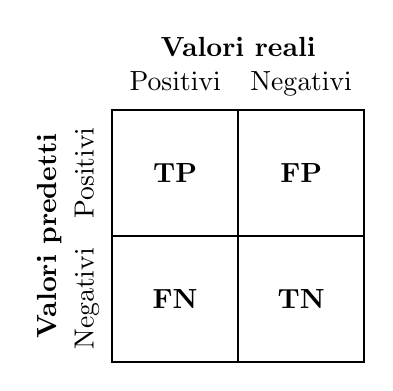
\begin{tikzpicture}[scale=0.8]
    
        \draw[thick] (0,0) rectangle (4,4);
        \draw[thick] (2,0) -- (2,4);
        \draw[thick] (0,2) -- (4,2);

        \node[above] at (2,4.7) {\textbf{Valori reali}};
        \node[rotate=90] at (-1,2) {\textbf{Valori predetti}};

        \node[above] at (1,4.0) {\strut Positivi};
        \node[above] at (3,4.0) {\strut Negativi};

        \node[rotate=90] at (-0.4,3) {\strut Positivi};
        \node[rotate=90] at (-0.4,1) {\strut Negativi};

        \node at (1,3) {\textbf{TP}};
        \node at (3,3) {\textbf{FP}};
        \node at (1,1) {\textbf{FN}};
        \node at (3,1) {\textbf{TN}};
    \end{tikzpicture}
\end{center}
    \caption{Matrice di confusione nel caso della classificazione binaria.}
    \label{fig:confusion-matrix}
\end{figure}

Ciascuna istanza classificata dal modello rientra in esattamente una delle quattro categorie racchiuse nella matrice di confusione.
\begin{itemize}
    \item Veri positivi ($\text{TP}$): istanze classificate correttamente come positive.
    \item Falsi positivi ($\text{FP}$): istanze classificate erroneamente come positive.
    \item Veri negativi ($\text{TN}$): istanze classificate correttamente come negative.
    \item Falsi negativi ($\text{FN}$): istanze classificate erroneamente come negative.
\end{itemize}

A partire dalla matrice di confusione, possiamo introdurre due metriche fondamentali nei problemi di classificazione binaria.
\begin{description}
    \item[Tasso di falsi positivi (\textit{False Positive Rate}, FPR)] È definito come il rapporto tra il numero di falsi positivi (FP) e il numero totale di istanze che appartengono effettivamente alla classe negativa:
    \begin{equation}
        \text{FPR} = \frac{\text{FP}}{\text{TN}+\text{FP}} .
    \end{equation}
    È quindi una misura di quanto frequentemente il modello sbagli nel classificare istanze negative come positive.
    
    \item[Tasso di falsi negativi (\textit{False Negative Rate}, FNR)] Analogamente al FPR, si può definire il FNR come
    \begin{equation}
        \text{FNR} = \frac{\text{FN}}{\text{TP}+\text{FN}} \enspace.
    \end{equation}
    In modo analogo al FPR, il FNR rappresenta una misura della frequenza con cui il modello classifichi erroneamente istanze positive come negative.
\end{description}
È importante evidenziare come FPR e FNR siano spesso in mutua competizione. 
Infatti, se si vuole ridurre il FNR, un modo per farlo è rendere il modello più ``inclusivo" nei confronti della classe positiva, anche a costo di classificare come positivi esempi che non lo sono, aumentando dunque il FPR. Lo stesso vale nel caso in cui si voglia ridurre il FPR.
Considerando un caso estremo ma esplicativo, un modo semplice per ottenere FPR = 0 è classificare ogni esempio come negativo, ma ciò comporta FNR = 1 (chiaramente, se sono presenti esempi di entrambe le classi).




\subsection{Overfitting e Underfitting}
\label{par:overfitting-underfitting}

\begin{figure}
    \centering
    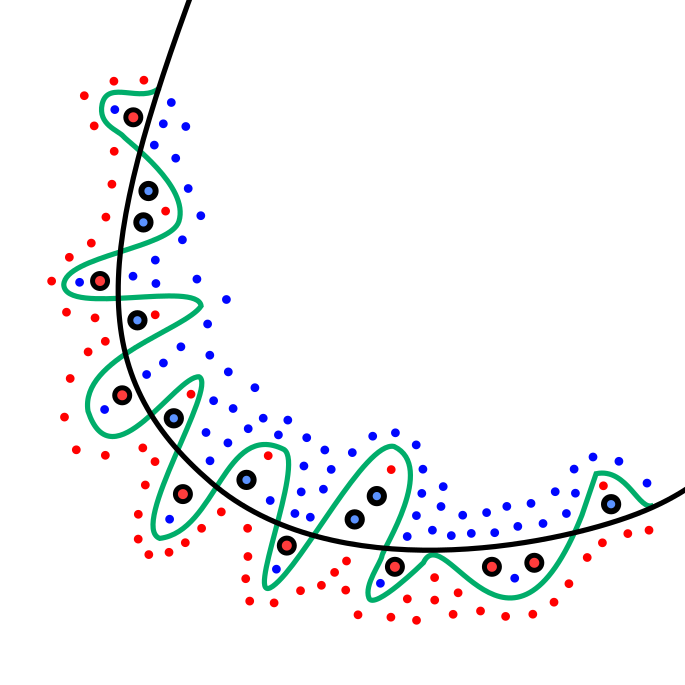
\includegraphics[width=0.5\linewidth]{images/overfitting.png}
    \caption{Due modelli (verde e nero) in un problema di classificazione binaria. Fonte: Chabacano, CC BY-SA 4.0 [https://creativecommons.org/licenses/by-sa/4.0].}
    \label{fig:overfitting}
\end{figure}

La Figura \ref{fig:overfitting} illustra un problema di classificazione binaria. Ciascuna osservazione corrisponde a un punto nel piano, che può appartenere alla classe blu oppure alla classe rossa. Si vuole quindi giungere a un classificatore in grado di predire, data un'osservazione, la classe di appartenenza. In questo caso, un classificatore non è altro che una funzione a due variabili, e l'obiettivo è trovare quella che meglio separa i punti blu da quelli rossi. Nella Figura \ref{fig:overfitting} ne sono illustrate due: una nera, che chiamiamo $\gamma$ e una verde, $\phi$.\\
I punti non contornati sono quelli utilizzati dall'algoritmo di addestramento, e fanno quindi parte del cosiddetto \textit{train set}, che indichiamo con $A$. I punti contornati, invece, rappresentano istanze nuove, non incontrate durante l'allenamento.

Chiaramente, la curva ideale sarebbe $\gamma$, che separa discretamente bene le osservazioni appartenenti a $A$ e perfettamente quelle nuove. Di certo, non potremmo affermare che $\phi$ sia un buon modello, in quanto non classifica correttamente neanche una delle osservazioni nuove. Eppure, se lo valutassimo solo su $A$, otterrebbe risultati migliori rispetto a $\gamma$. Quello esemplificato da $\phi$ è un fenomeno ben noto, chiamato \textit{overfitting}, dal quale ci si deve guardare in qualsiasi problema di ML. Infatti, $\phi$ si è specializzato eccessivamente su $A$, adattandosi alle caratteristiche peculiari dei suoi esempi che non avevano niente a che vedere con la relazione generale sottostante ai dati, e dunque non è in grado di \textit{generalizzare} su dati mai visti (cosa che $\gamma$ è in grado di fare).\\
Per questa ragione, valutare le performance di un modello solamente sul train set non basta per comprenderne la bontà: bisogna ricorrere a un \textit{test set} $T$, cioè un insieme di dati disgiunto da $A$.

Nonostante buone prestazioni sul train set non implichino la qualità del modello, rappresentano comunque una condizione necessaria per raggiungerla. Infatti, prestazioni scarse su $A$ indicano che il modello utilizzato non è abbastanza espressivo/potente per il dato problema (fenomeno di \textit{underfitting}). \\
Considerando nuovamente l'esempio della Figura \ref{fig:overfitting}, una retta rappresenterebbe un modello troppo poco espressivo per i dati presenti (nessuna funzione lineare separerebbe efficacemente i punti blu da quelli rossi), e soffrirebbe dunque di underfitting. Di fatto, avrebbe certamente prestazioni molto scarse già sul train set e a maggior ragione sul test set.

Nel Paragrafo \ref{par:tecniche-di-stima} presenteremo alcune tecniche con cui è possibile ricavare, a partire da un dataset, un train set e un test set disgiunto da esso.

\subsection{Tecniche di Stima delle Prestazioni}
\label{par:tecniche-di-stima}
Per quanto visto nel paragrafo precedente, è opportuno suddividere il dataset iniziale $D = \{(\mathbf{x}_1, y_1), \dots, (\mathbf{x}_n, y_n)\}$ in un train set $A$ e un test set $T$, garantendone la disgiunzione. \\
È fondamentale anche che entrambi $A$ e $T$ mantengano la distribuzione di $D$, poiché quest'ultimo rappresenta un campione della popolazione e, di conseguenza, ne rispecchia il profilo statistico (dovrebbe sempre farlo). Le tecniche di \textit{campionamento stratificato} servono proprio a fare in modo che qualsiasi sottoinsieme ricavato da $D$ ne rifletta la distribuzione. \\
Se $A$ e $T$ avessero distribuzioni diverse, staremmo valutando il modello su una popolazione distribuita diversamente rispetto a quella su cui è stato allenato. 

Prendiamo come esempio un problema di classificazione binaria. Supponiamo di avere $D$ contenente 500 esempi positivi e 500 esempi negativi, e di volerlo partizionare (tecnica che prende il nome di \textit{holdout}, come vedremo tra breve) in un train set $A$ con il 70\% degli esempi e un test set $T$ con il 30\% degli esempi. In tal caso, un metodo di campionamento stratificato garantirà che $A$ contenga 350 esempi positivi e 350 esempi negativi, e che $T$ contenga 150 esempi positivi e 150 esempi negativi.

Assumeremo sempre che qualsiasi sottoinsieme ricavato da $D$ sia correttamente stratificato.

\subsubsection{Holdout}
Come già accennato, la metodologia holdout consiste nell'approccio più intuitivo possibile: partizionare $D$, ossia nel suddividerlo in un train set $A$ e in un test set $T$, in modo tale che $D = T \cup A $ e $ T \cap A = \emptyset$. Nella Figura \ref{fig:holdout} è presente una visualizzazione grafica di questa metodologia.

\begin{figure}[h]
    \centering
    \begin{center}
    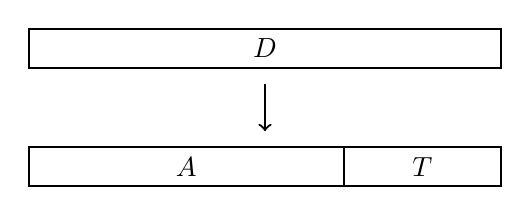
\begin{tikzpicture}
        \draw[thick] (0,3) rectangle (6,3.5);
        \node at (3,3.25) {\textbf{$D$}};

        \draw[thick,->] (3,2.8) -- (3,2.2);

        \draw[thick] (0,1.5) rectangle (6,2);
        \draw[thick] (4,1.5) -- (4,2);

        \node at (2,1.75) {\textbf{$A$}};
        \node at (5,1.75) {\textbf{$T$}};
    \end{tikzpicture}
\end{center}
    \caption{Visualizzazione grafica del metodo holdout.}
    \label{fig:holdout}
\end{figure}

Chiaramente, è necessario scegliere quanti degli esempi di $D$ inserire in $A$ e, di conseguenza, quanti in $T$. Di fatto, il rapporto $|A|/|D|$, e quindi $|T|/|D|$, è un aspetto critico del metodo holdout.
Aumentando la dimensione di $A$, le prestazioni del modello dovrebbero migliorare; tuttavia, la conseguente riduzione di $T$ porterebbe a un maggior errore nella stima della bontà di generalizzazione. Viceversa, aumentando la dimensione di $T$, la valutazione delle prestazioni sarebbe più accurata, ma la qualità delle risposte del modello ne risentirebbe.
Non esiste una soluzione perfetta a questo dilemma; è necessario un compromesso. Una pratica comune è
scegliere $|A|/|D| = 2/3$ oppure $|A|/|D| = 4/5$.

Mantenendo invariato il numero di esempi in $A$ (e di conseguenza in $T$), è possibile generare più coppie $(A,T)$ a partire dallo stesso dataset $D$, permutando gli esempi in modo casuale (curando sempre la stratificazione). In pratica, si eseguono $n$ holdout \textit{ripetuti} (ad esempio, 100), allenando e valutando altrettanti modelli, ciascuno su una coppia $(A,T)$ distinta, sempre derivata da $D$. \\
Per ottenere una valutazione complessiva, si calcola la media delle $n$ valutazioni ottenute. 

Successivamente, se la valutazione complessiva ottenuta è soddisfacente, si utilizza come train set l'intero dataset $D$ per ri-addestrare un ultimo modello, quello definitivo che verrà effettivamente impiegato. L'assunzione di fondo, generalmente corretta, è che allenando un modello con più dati, le sue prestazioni migliorino (o che sicuramente non peggiorino). L'operazione di \textit{ri-allenamento} finale svolta sull'intero dataset prende il nome di \textit{refit}, e viene sempre svolta, ammesso che la valutazione finale sia sufficientemente buona.

\subsubsection{Cross-validation}
La metodologia cross-validation (CV) (\cite{stone1974cross}) prevede di suddividere $ D $ in $ k $ sottoinsiemi di cardinalità uguale o simile, tali che 
\begin{equation}
    \begin{cases}
        D = \bigcup_{i=1}^{k} D_i \\
        D_i \cap D_j = \emptyset \quad \forall i, j \in \{1, \dots, k\}, \; i \neq j \enspace .
    \end{cases}
\end{equation}
In altre parole, i $k$ sottoinsiemi devono costituire una partizione di $D$.

Si effettuano $k$ iterazioni; a ogni iterazione, uno dei sottoinsiemi $D_i$ non ancora utilizzato come test set viene selezionato a tale scopo, mentre tutti i rimanenti sottoinsiemi vanno a costituire il training set, come illustrato in Figura \ref{fig:cross-validation}.  

Al termine delle iterazioni, si dispone di $k$ valutazioni, la cui media rappresenta la valutazione complessiva.  

Dal momento che la stabilità e l'accuratezza della CV dipendono fortemente dal valore di $k$, questa tecnica è nota anche come \textit{$k$-fold cross-validation}. Alcuni valori comuni per $k$ sono 3, 5 e 10.

\begin{figure}[h]
    \centering
    \begin{center}
    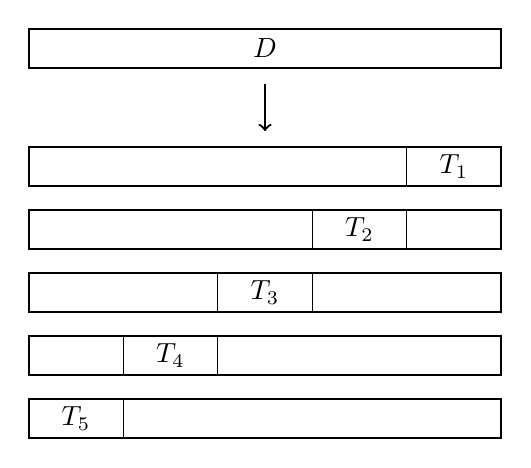
\begin{tikzpicture}
        \draw[thick] (0,6) rectangle (6,6.5);
        \node at (3,6.25) {$D$};

        \draw[thick,->] (3,5.8) -- (3,5.2);

        \foreach \y in {4.5,3.7,2.9,2.1,1.3} {
            \draw[thick] (0,\y) rectangle (6,\y+0.5);
        }

        \draw (4.8,4.5) rectangle (6,5);
        \draw (3.6,3.7) rectangle (4.8,4.2);
        \draw (2.4,2.9) rectangle (3.6,3.4);
        \draw (1.2,2.1) rectangle (2.4,2.6);
        \draw (0,1.3) rectangle (1.2,1.8);

        \node at (5.4,4.75) {$T_1$};
        \node at (4.2,3.95) {$T_2$};
        \node at (3,3.15) {$T_3$};
        \node at (1.8,2.35) {$T_4$};
        \node at (0.6,1.55) {$T_5$};

    \end{tikzpicture}
    \end{center}
    \caption{Una visualizzazione delle 5 suddivisioni diverse che si ottengono nella 5-fold CV.}
    \label{fig:cross-validation}
\end{figure}

L'intero processo di $k$-fold CV può essere ripetuto $p$ volte, permutando a ogni iterazione gli esempi di $D$ in maniera casuale per ridurre la dipendenza della valutazione dalla specifica suddivisione iniziale del dataset. Al termine delle iterazioni, si restituisce la media delle $p$ valutazioni ottenute. Un caso possibile è la \textit{10-times 10-fold CV}.

Una tipologia speciale di CV è la \textit{Leave-One-Out} (LOO), in cui si fissa $k = |D|$. Le valutazioni che ne risultano sono molto accurate, ma il costo computazionale dell'addestramento di $|D|$ modelli può essere proibitivo per dataset di grandi dimensioni.


\subsection{Tuning degli Iperparametri}
Mentre per i parametri di un modello i valori ottimali vengono definiti dall'algoritmo di addestramento, per gli iperparametri (vedi Paragrafo \ref{par:tassonomia}) è necessaria una apposita fase di \textit{tuning} (\cite{feurer2019hpo}). 

Di seguito, illustriamo un approccio molto diffuso per via della sua semplicità, che prende il nome di \textit{grid search}.

Consideriamo un modello avente $h$ iperparametri, con indice $i \in \{1,2, \dots, h \}$. Per ciascun iperparametro $i$, fissiamo un insieme di $v_i$ valori con cui sperimentare. È fondamentale scegliere con cura tali valori per evitare che il numero totale di combinazioni da esaminare, che indichiamo con $C$, cresca eccessivamente. Infatti, si ha:
\begin{equation}
    C = \prod_{i=1}^h v_i \enspace .
\end{equation}
Per ogni combinazione, si addestra e si valuta un modello; si sceglie poi quello con la performance migliore. Indichiamo con $c^*$ la combinazione di tale modello.

Come già discusso nel Paragrafo \ref{par:overfitting-underfitting}, non possiamo misurare le prestazioni limitandoci ad $A$. Dunque, per scegliere il modello migliore tra i $C$ generati, ricorriamo a un apposito \textit{validation set} $V$, ricavato da $D$ ma disgiunto da $A$ e da $T$.
Viene poi generato un modello $m$ con la combinazione $c^*$, allenandolo sull'unione $A \cup V$ (primo refit).  
Infine, si utilizza un apposito test set $T$ per valutare le performance di $m$. Se sono soddisfacenti, si effettua un secondo refit su $A \cup V \cup T$, ossia su $D$.

Un altro approccio possibile consiste nella \textit{random search}, che si basa su una ricerca casuale nello spazio delle combinazioni possibili (\cite{bergstra2012random}).

Nel Paragrafo \ref{par:tecniche-di-stima} abbiamo illustrato come valutare le prestazioni di un modello suddividendo il dataset $D$ nei sottoinsiemi $A$ e $T$. Tuttavia, non abbiamo considerato il caso in cui sia necessario eseguire il tuning degli iperparametri, introducendo quindi un ulteriore sottoinsieme, $V$.  

In questo scenario, le suddivisioni seguono una struttura annidata: una prima suddivisione esterna separa $D$ in $A$ e $T$, mentre una successiva suddivisione interna suddivide $A$ in un sottoinsieme di training ridotto e in $V$.  
Queste operazioni possono essere effettuate con lo stesso metodo (ad esempio, holdout-holdout), oppure con tecniche differenti, come nel caso di holdout seguito da CV. La Figura \ref{fig:cv-annidata} illustra una visualizzazione di quest'ultimo approccio.

\begin{figure}[h]
    \centering
    \begin{center}
    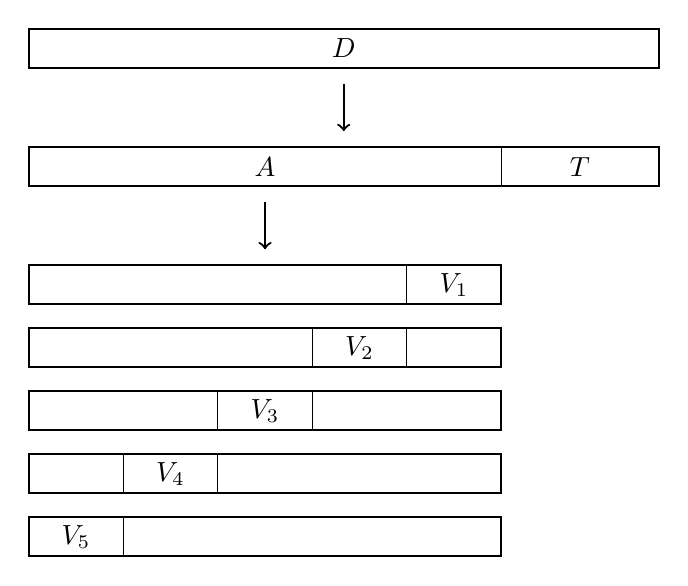
\begin{tikzpicture}
        \draw[thick] (0,7.5) rectangle (8, 8);
        \node at (4,7.75) {$D$};
        \draw[thick,->] (4,7.3) -- (4,6.7);
     
        \draw[thick] (0,6) rectangle (8,6.5);
        \node at (3,6.25) {$A$};
        \draw (6,6) -- (6,6.5);
        \node at (7,6.25) {$T$};

        \draw[thick,->] (3,5.8) -- (3,5.2);

        \foreach \y in {4.5,3.7,2.9,2.1,1.3} {
            \draw[thick] (0,\y) rectangle (6,\y+0.5);
        }

        \draw (4.8,4.5) rectangle (6,5);
        \draw (3.6,3.7) rectangle (4.8,4.2);
        \draw (2.4,2.9) rectangle (3.6,3.4);
        \draw (1.2,2.1) rectangle (2.4,2.6);
        \draw (0,1.3) rectangle (1.2,1.8);

        \node at (5.4,4.75) {$V_1$};
        \node at (4.2,3.95) {$V_2$};
        \node at (3,3.15) {$V_3$};
        \node at (1.8,2.35) {$V_4$};
        \node at (0.6,1.55) {$V_5$};

    \end{tikzpicture}
\end{center}
    \caption{In questo esempio, ciascuna configurazione di iperparametri viene valutata con una 5-fold CV annidata svolta su $A$, mentre la valutazione finale del modello viene effettuata su un test set esterno $T$ ricavato da $D$ tramite holdout.}
    \label{fig:cv-annidata}
\end{figure}

Un caso di particolare interesse si verifica quando la cross-validation viene utilizzata per la suddivisione esterna. A ciascuna iterazione esterna corrisponde un train set distinto, il che implica l'addestramento di un modello differente, con iperparametri ottimali che possono variare rispetto a quelli ottenuti nelle altre iterazioni. Di conseguenza, ogni iterazione esterna può generare un modello con una configurazione di iperparametri unica. In questo scenario, il modello finale può essere selezionato casualmente tra quelli addestrati.








\section{Tipologie di Modello}
\label{par:tipologie}
Presentiamo brevemente le famiglie di modelli di cui ci serviremo nei capitoli successivi.

\subsection{Support Vector Machine Lineari}
\label{par:svm}
Le Support Vector Machine (SVM) sono state proposte da \textcite{cortes1995svm} come una classe di algoritmi di apprendimento automatico utilizzabili principalmente per problemi di classificazione e di regressione. L'idea centrale delle SVM è quella di identificare un iperpiano ottimale che separi le istanze di dati appartenenti a classi differenti. \\
In questo paragrafo ci concentriamo sulle SVM lineari nel contesto della classificazione binaria.

Sia $D$ un dataset composto da $n$ esempi:
\begin{equation}
    D = \{ (\mathbf{x}_i, y_i) \in \mathbb{R}^d \times \{-1,+1 \}, \enspace i \in \{1,2, \dots, n \} \}.
\end{equation}
Ciascuna osservazione $\mathbf{x}_i$ è un vettore in $\mathbb{R}^d$ che rappresenta un punto in uno spazio a $d$ dimensioni, 
mentre $y_i$ è l’etichetta associata all’istanza, appartenente all’insieme $\{-1, +1\}$. Siamo quindi in un contesto di classificazione binaria.

L'idea di base è trovare nello spazio delle osservazioni un iperpiano in grado di separare istanze di classi diverse (se possibile, ossia se le istanze sono \textit{linearmente separabili}). Di iperpiani con questa caratteristica ce ne sono infiniti, per via della continuità di $\mathbb{R}^d$. Tuttavia, noi desideriamo quello più tollerante a piccole perturbazioni nei dati, ossia quello con la maggior capacità di generalizzazione. 

Facendo riferimento all'esempio bidimensionale della Figura \ref{fig:hyperplanes}, l'iperpiano (in questo caso, la retta) ideale sarebbe $H_1$, in quanto è poco probabile che piccole variazioni nelle posizioni delle osservazioni compromettano la correttezza della classificazione. $H_1$, oltre a separare correttamente le istanze in base alla classe, si mantiene alla massima distanza possibile da qualsiasi punto. Questo lo rende l'iperpiano ottimale. Al contrario, $H_2$ è molto suscettibile a piccole fluttuazioni delle osservazioni, in quanto vi si mantiene vicino.

\begin{figure}[ht]
    \centering
    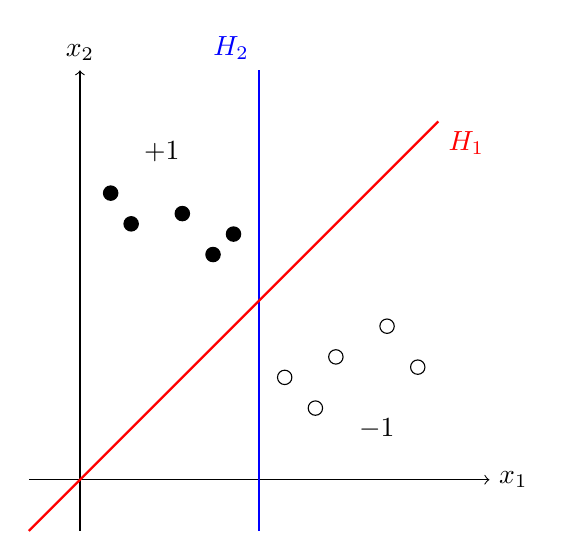
\begin{tikzpicture}[scale=1.3]
    
        \draw[->] (-0.5,0) -- (4,0) node[right] {$x_1$};
        \draw[->] (0,-0.5) -- (0,4) node[above] {$x_2$};
    
        \foreach \x/\y in {0.3/2.8, 0.5/2.5, 1/2.6, 1.3/2.2, 1.5/2.4} {
            \filldraw[black] (\x,\y) circle (2pt);
        }
        
        \foreach \x/\y in {2/1, 2.3/0.7, 2.5/1.2, 3/1.5, 3.3/1.1} {
            \draw[black] (\x,\y) circle (2pt);
        }
    
        \draw[blue, thick] (1.75,-0.5) -- (1.75,4) node[above left] {$H_2$};
    
        \draw[red, thick] (-0.5,-0.5) -- (3.5,3.5) node[below right] {$H_1$};
    
        \node at (0.8,3.2) {$+1$};
        \node at (2.9,0.5) {$-1$};

    \end{tikzpicture}
    \caption{Un problema di classificazione binaria bidimensionale, con due possibili rette separatrici, $H_1$ e $H_2$.}
    \label{fig:hyperplanes}
\end{figure}

Se le osservazioni sono linearmente separabili, possiamo trovare due iperpiani paralleli $H^+$ e $H^-$ che separino correttamente le due classi, in modo tale che la distanza tra essi sia massima. L'iperpiano ottimale giace esattamente a metà tra $H^+$ e $H^-$. \\
La Figura \ref{fig:svm-margin} aiuta a visualizzare tutti e tre gli iperpiani di cui sopra con un esempio bidimensionale.

Possiamo descrivere i due iperpiani $H^+$ e $H^-$ con le seguenti equazioni: 

\begin{equation}
    \begin{aligned}
        H^+ &: \mathbf{w}^{\top} \mathbf{x}+b=+1 \\
        H^- &: \mathbf{w}^{\top} \mathbf{x}+b=-1 \enspace .
    \end{aligned}
\end{equation}

Stiamo dunque chiedendo che, per qualsiasi esempio $(\mathbf{x}_i, y_i) \in D$, valga:

\begin{equation}
    \begin{cases}
        \mathbf{w}^{\top} \mathbf{x}_i +b \geq +1, \quad \text{se } y_i=+1, \\
        \mathbf{w}^{\top} \mathbf{x}_i +b \leq -1, \quad \text{se }y_i=-1 \enspace .
    \end{cases}
\end{equation}
Possiamo sintetizzare questi vincoli imponendo
\begin{equation}
    y_i(\mathbf{w}^{\top} \mathbf{x}_i +b) \geq 1, \quad \forall \space i \in \{1, \dots, n\} \enspace .
\end{equation}

La distanza tra $H^+$ e $H^-$, nota come \textit{margine}, può essere espressa come
\begin{equation}
    \frac{2}{\|\mathbf{w}\|} \enspace ,
\end{equation}
ed è proprio la quantità che vogliamo massimizzare.

\begin{figure}[ht]
    \centering
    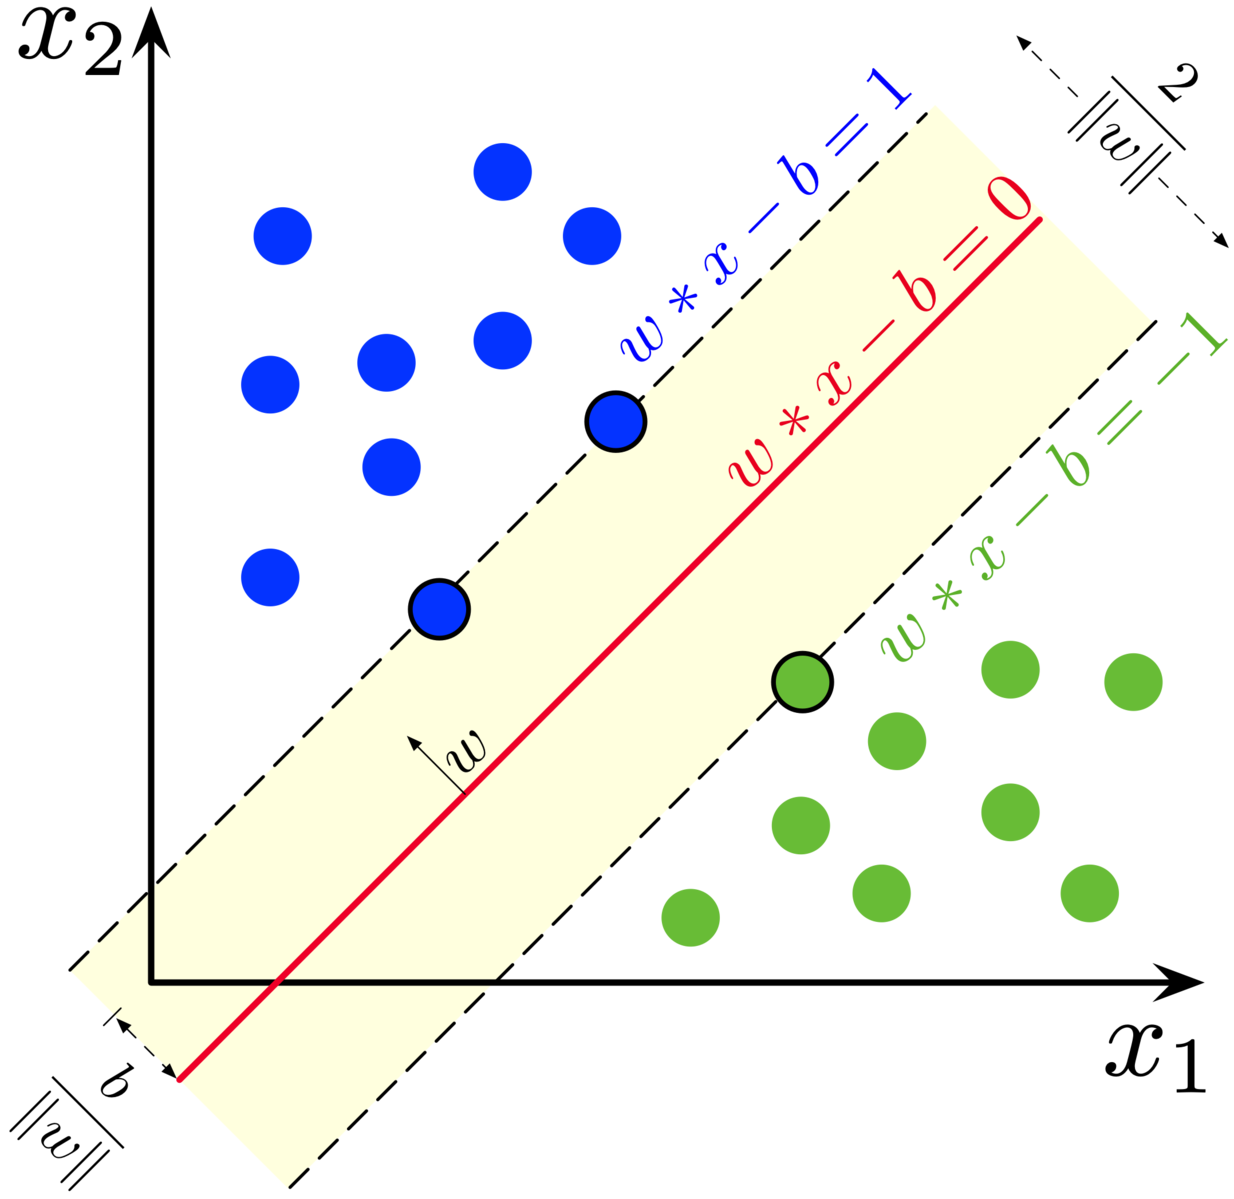
\includegraphics[width=0.5\linewidth]{images/svm-margin.png}
    \caption{I due iperpiani (rette) di margine massimo e l'iperpiano separatore che vi giace in mezzo. In questo esempio, $b$ è preceduto da un segno negativo, diversamente da quanto scritto finora; si tratta di formulazioni equivalenti. Fonte: Larhmam, CC BY-SA 4.0 [https://creativecommons.org/licenses/by-sa/4.0].}
    \label{fig:svm-margin}
\end{figure}

Tenuto conto che massimizzare $\|\mathbf{w}\|^{-1}$ equivale a minimizzare $\|\mathbf{w}\|^2$, possiamo scrivere il problema di ottimizzazione a cui siamo giunti in questo modo:
\begin{equation}
    \begin{aligned}
    \min_{\mathbf{w},b} \quad & \frac{1}{2}\|\mathbf{w}\|^2 \\
    \text{s.t.} \quad & y_i(\mathbf{w}^{\top} \mathbf{x}_i +b) \geq 1, \quad \forall \space i \in \{1, \dots, n\} \enspace .
    \end{aligned}
    \label{expr:primal-hard-margin}
\end{equation}

È importante notare che l'iperpiano separatore ottimale è completamente determinato dai punti $\mathbf{x}_i$ che si trovano più vicini a esso, come evidenziato in Figura \ref{fig:svm-margin}. Questi $\mathbf{x}_i$ sono chiamati \textit{support vector} (da cui il nome della famiglia di modelli).

Il problema di ottimizzazione vincolata (\ref{expr:primal-hard-margin}) riguarda il caso \textit{hard margin}, ossia quello in cui le osservazioni sono linearmente separabili. Comunemente, però, ciò non accade, e quindi si adotta un approccio \textit{soft margin}, nel quale si tollera che la SVM commetta qualche errore, permettendo la violazione del vincolo $y_i(\mathbf{w}^{\top} \mathbf{x}_i +b) \geq 1$ per qualche $i$.

A questo scopo, modifichiamo (\ref{expr:primal-hard-margin}) introducendo delle variabili \textit{di slack} $\xi_i$:
\begin{equation}
    \begin{aligned}
    \min_{\mathbf{w},b} \quad & \frac{1}{2}\|\mathbf{w}\|^2 + C \sum_{i=1}^n \xi_i \\
    \text{s.t.} \quad & y_i(\mathbf{w}^{\top} \mathbf{x}_i +b) \geq 1 - \xi_i, \\
    & \xi_i \geq 0, \quad \forall \space i \in \{1, \dots, n\} \enspace .
    \end{aligned}
    \label{expr:primal-soft-margin}
\end{equation}

Grazie a questa nuova formulazione, ciascuna $\xi_i$ vale più di 0 solo se l'osservazione $i$-esima vìola il vincolo $y_i(\mathbf{w}^{\top} \mathbf{x}_i +b) \geq 1$. Dunque, la somma di tutte le $\xi_i$ quantifica la violazione complessiva del suddetto vincolo. Penalizzando la funzione obiettivo originale in (\ref{expr:primal-hard-margin}) con questa somma, moltiplicata per una costante $C>0$ (che sarà un iperparametro), modelliamo il caso soft margin. All'aumentare di $C$, la penalizzazione pesa maggiormente sull'obiettivo; di conseguenza, la SVM tollera sempre meno gli errori.

Sfruttando i moltiplicatori di Lagrange, possiamo passare al \textit{problema duale} di (\ref{expr:primal-soft-margin}):
\begin{equation}
    \begin{aligned}
    \max_{\boldsymbol{\alpha}} \quad & \sum_{i=1}^{n} \alpha_i - \frac{1}{2} \sum_{i=1}^{n} \sum_{j=1}^{n} \alpha_i \alpha_j y_i y_j \mathbf{x}_i^{\top} \mathbf{x}_j \\
    \text{s.t.} \quad & \sum_{i=1}^{n} \alpha_i y_i = 0, \\
    & 0 \leq \alpha_i \leq C, \quad \forall \space i \in \{1, \dots, n\} \enspace .
    \end{aligned}
\end{equation}
Dal momento che si tratta di un problema di ottimizzazione non lineare vincolata, vanno soddisfatte le condizioni di Karush-Kuhn-Tucker (KKT):
\begin{equation}
        \begin{cases}
            \alpha_i \geq 0, \quad \mu_i \geq 0, \\
            y_i f(\mathbf{x}_i)-1 + \xi_i \geq 0, \\
            \alpha_i (y_i f(\mathbf{x}_i)-1 + \xi_i) = 0, \\
            \xi_i \geq 0, \quad \mu_i \xi_i = 0 \enspace ,
        \end{cases}
\end{equation}
dove $f(\mathbf{x}) = \mathbf{w}^{\top} \mathbf{x} +b$; ossia, $f(\mathbf{x})$ è l'espressione dell'iperpiano separatore.

Dalle KKT evinciamo che, per qualsiasi esempio $(\mathbf{x}_i, y_i) \in D$:
\begin{itemize}
    \item se $\alpha_i =0$, allora $y_i f(\mathbf{x}_i)-1 + \xi_i$ può assumere qualsiasi valore; in altre parole, l'esempio $i$-esimo non ha influenza sull'iperpiano.

    \item Se $\alpha_i > 0$, allora necessariamente si ha $y_i f(\mathbf{x}_i) = 1 -\xi_i$, ossia: $\mathbf{x}_i$ contribuisce a determinare l'iperpiano ed è quindi un support vector.
\end{itemize}

\subsubsection{Variante Cost-Sensitive}

Finora abbiamo considerato una SVM classica, che tratta gli errori in maniera omogenea, senza distinzione tra FP e FN.
Tuttavia, come vedremo nei prossimi capitoli, è di nostro interesse poter attribuire una gravità diversa ai FP rispetto che ai FN, per poter regolare il FPR e, di conseguenza, il FNR di una SVM (ricordiamo che, come sottolineato nel Paragrafo \ref{par:metriche}, FP e FN sono generalmente in mutua competizione). Infatti, ciò che si vuole ottenere è una SVM \textit{cost-sensitive} che tolleri più errori di un tipo (ad esempio, FP), ma meno dell'altro.

A tale scopo, un possibile approccio proposto da \textcite{morik:1999:svm} consiste nel separare la sommatoria della funzione obiettivo di (\ref{expr:primal-soft-margin}) per distinguere la penalizzazione dovuta ai FP da quella dovuta ai FN, e moltiplicare ciascuna per il proprio fattore di costo, rispettivamente $C_+$ e $C_-$ (questi ultimi sono a tutti gli effetti degli iperparametri). Si ottiene:
\begin{equation}
    \begin{aligned}
    \min_{\mathbf{w},b} \quad & \frac{1}{2}\|\mathbf{w}\|^2 + C_+ \sum_{i:y_i=+1}^n \xi_i + C_- \sum_{i:y_i=-1}^n \xi_i \\
    \text{s.t.} \quad & y_i(\mathbf{w}^{\top} \mathbf{x}_i +b) \geq 1 - \xi_i, \\
    & \xi_i \geq 0, \quad \forall \space i \in \{1, \dots, n\} \enspace .
    \end{aligned}
\end{equation}
Se $C_+ > C_-$, gli errori commessi sugli esempi positivi, ossia i FN, gravano maggiormente sull'obiettivo rispetto ai FP, dunque la SVM tenderà a commettere meno FN e più FP. Se, invece, $C_+ < C_-$, la SVM commetterà meno FP e più FN.
Il caso in cui $C_+ = C_-$ ci riporta al problema originale, in cui FP e FN hanno la stessa importanza.

Essenzialmente, $C_+ >0$ e $C_- >0$ hanno la stessa funzione dell'iperparametro $C$ introdotto nel caso non cost-sensitive, ma si occupano ciascuno di una delle due classi in maniera separata.









\subsection{Reti Neurali}
\label{par:nn}
Una rete neurale (\textit{Neural Net}, NN) è una tipologia di modello di ML ispirata alla struttura e al funzionamento del sistema nervoso centrale delle specie animali.

L'oggetto astratto alla base delle NN è il neurone artificiale (\cite{mcculloch1943}), schematizzato in Figura \ref{fig:neuron}. Ciascun neurone riceve uno o più input, ne effettua la somma pesata, ci aggiunge un termine costante $b$ noto come \textit{bias}, e sottopone il risultato a una \textit{funzione di attivazione} $\alpha$ per ottenere l'output $y$:
\begin{equation}
    y = \alpha \left(\sum_{j=1}^d w_j x_j + b \right) \enspace ,
    \label{expr:neuron-output}
\end{equation}
dove $d$ è il numero di input (e di conseguenza di pesi).

\begin{figure}[ht]
    \centering
    \begin{tikzpicture}

    \node (x1) at (0,1.5) {$x_1$};
    \node (x2) at (0,0.5) {$x_2$};
    \node (xdots) at (0,-0.5) {$\vdots$};
    \node (xn) at (0,-1.5) {$x_d$};

    \node (w1) at (1,1.5) {$w_1$};
    \node (w2) at (1,0.5) {$w_2$};
    \node (wdots) at (1,-0.5) {$\vdots$};
    \node (wn) at (1,-1.5) {$w_d$};
    
    \node[draw, circle, minimum size=1cm] (sum) at (3,0) {$\sum$};

    \node (b) at (2,-2) {$b$};
    \draw[->] (b) -- (sum);

    \node[draw, rectangle, minimum width=1.2cm, minimum height=0.8cm] (act) at (5,0) {$\alpha$};

    \node (y) at (7,0) {$y$};

    \draw[->] (x1) -- (sum);
    \draw[->] (x2) -- (sum);
    \draw[->] (xn) -- (sum);
    
    \draw[->] (sum) -- (act);
    \draw[->] (act) -- (y);

\end{tikzpicture}
    \caption{Un neurone artificiale.}
    \label{fig:neuron}
\end{figure}

Una tipica funzione di attivazione è la sigmoide (il cui grafico è illustrato in Figura \ref{fig:sigmoid}):
\begin{equation}
    \alpha(x) = \frac{1}{1+e^{-x}} \enspace .
\end{equation}

\begin{figure}[ht]
    \centering
    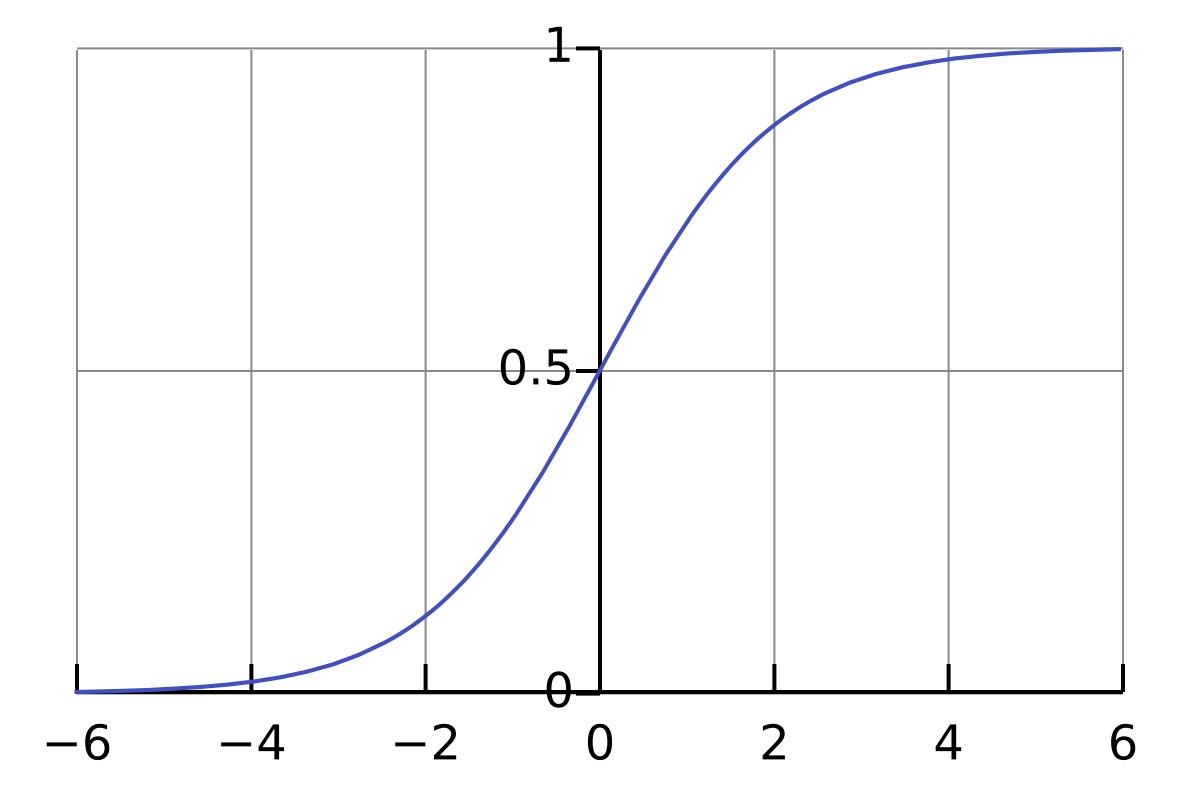
\includegraphics[width=0.5\linewidth]{images/sigmoid.png}
    \caption{La funzione sigmoide.}
    \label{fig:sigmoid}
\end{figure}

Più neuroni possono essere collegati a formare una NN come quella in Figura \ref{fig:neural-net} (\cite{zhou2021ml}). Si tratta di una tipica rete a più strati, in cui ogni neurone di ogni strato è connesso con tutti quelli dello strato successivo. I neuroni facenti parte dello stesso strato o di strati non adiacenti, invece, non sono connessi. NN di questo tipo prendono il nome di reti neurali multistrato \textit{feedforward}, perché l'informazione, durante la classificazione di un'istanza, viaggia solamente \textit{in avanti}: partendo dallo strato di input, attraversa uno a uno gli strati nascosti per poi giungere allo strato di output. Quest'ultimo, in un problema di classificazione binaria, è composto da un solo neurone, il cui output è un valore $o$ nell'intervallo continuo $[0,1]$. Tale valore viene confrontato con una soglia $\tau \in [0,1]$: l'osservazione $\mathbf{x}$ viene classificata come positiva se e solo se $o_{\mathbf{x}} > \tau$.

Ciascun neurone si comporta allo stesso modo, producendo un output secondo (\ref{expr:neuron-output}). \\
Per la precisione, lo strato di input non è composto da neuroni: ogni nodo rappresenta semplicemente un attributo dell'osservazione, il cui valore va direttamente in input allo strato successivo.

\begin{figure}[h]
    \centering
    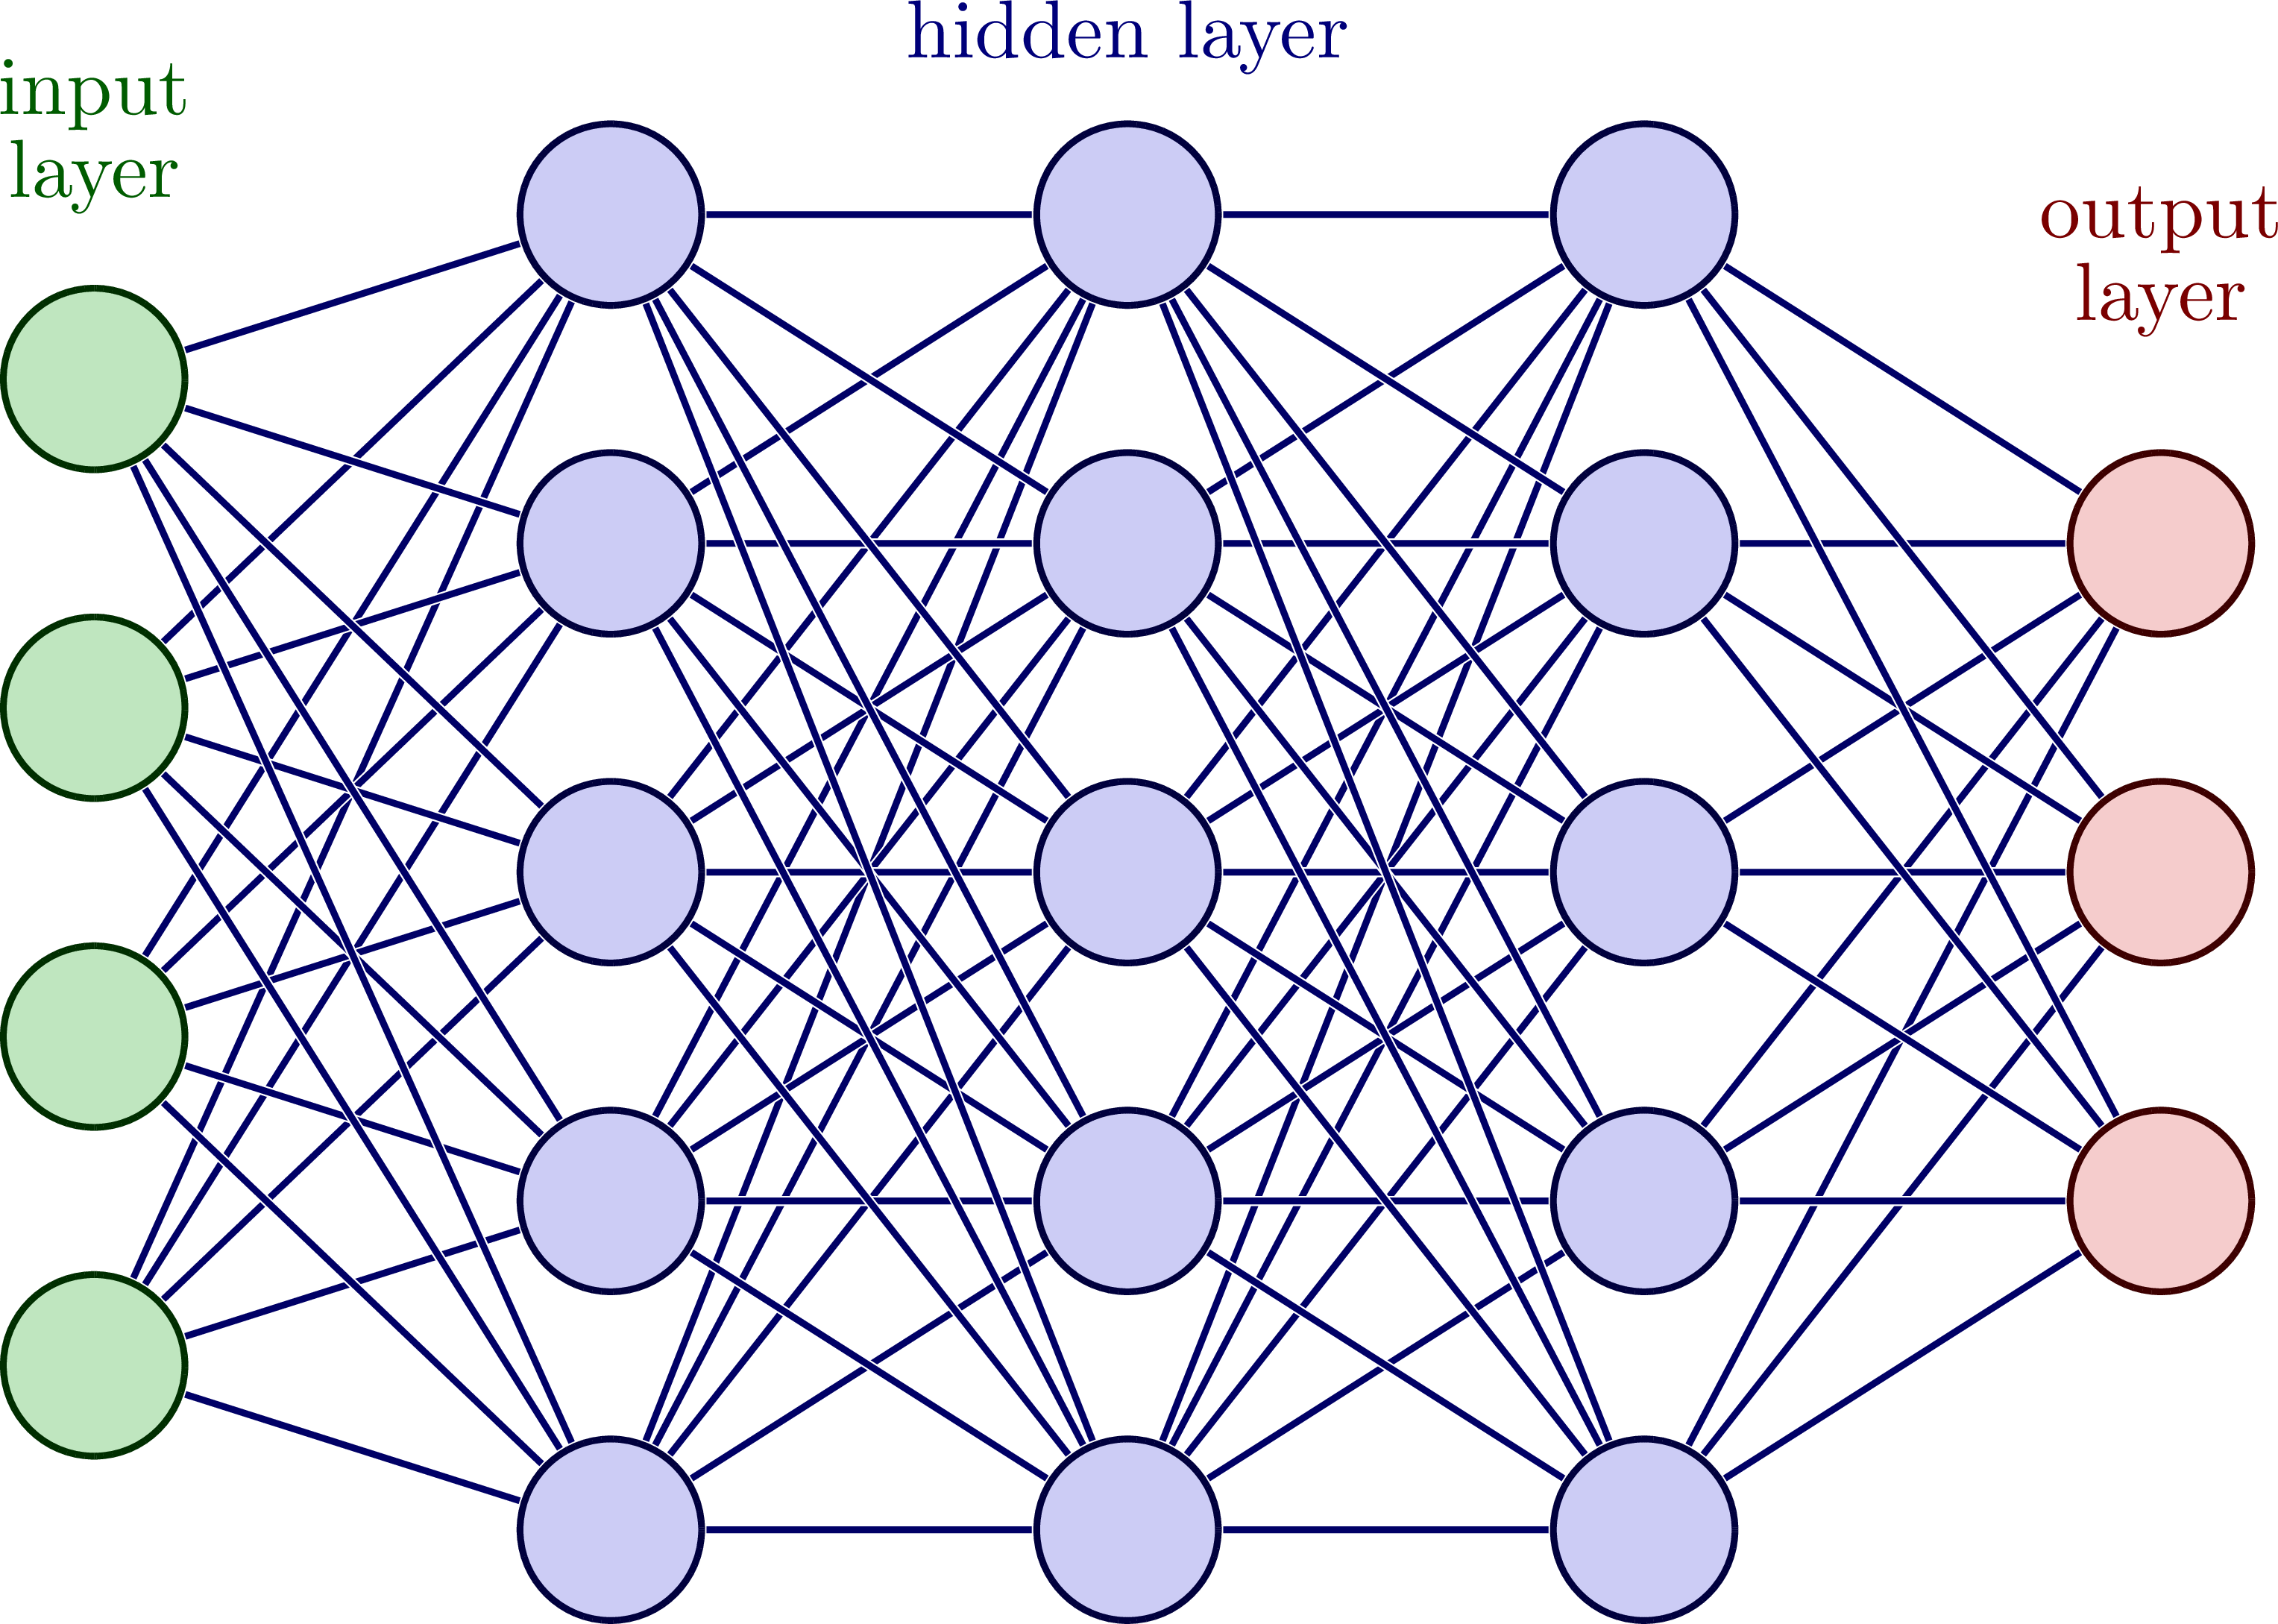
\includegraphics[width=0.6\linewidth]{images/neural-net.png}
    \caption{Una rete neurale \textit{feedforward}. Fonte: Izaak Neutelings, CC BY-SA 4.0 [https://creativecommons.org/licenses/by-sa/4.0].}
    \label{fig:neural-net}
\end{figure}

L'algoritmo di apprendimento delle NN ha come scopo trovare i valori ottimali dei pesi e dei bias, che sono quindi i parametri di questa tipologia di modello. Tale algoritmo si basa su una \textit{funzione di perdita} $L$ (dall'inglese \textit{loss}), che misura la discrepanza tra le previsioni del modello e i valori reali.

Una funzione comunemente utilizzata è l'errore quadratico medio (MSE), che per l'esempio $i$-esimo è definita come:
\begin{equation}
    L_i = \frac{1}{2} \sum_{k=1}^l (y_k^i - \hat{y}_k^i)^2
\end{equation}
dove $l$ è il numero di neuroni di output, $y_k^i$ è il valore che il $k$-esimo neurone di output dovrebbe restituire (facilmente ricavabile dall'etichetta $i$-esima) e $\hat{y}_k^i$ è il valore effettivo che tale neurone restituisce.

Da notare che ogni $L_i$ è in realtà una funzione dei pesi e dei bias della rete, in quanto sono questi a determinare ciascun $\hat{y}_k^i$. Quindi, per ciascun esempio, basterebbe calcolare il gradiente $\nabla L_i$, che ci dà la direzione di massimizzazione di $L_i$, e aggiornare i pesi e i bias della rete per muoversi nella direzione opposta. Questa è l'idea alla base dell'algoritmo di apprendimento delle NN, anche se quest'ultimo opera in realtà in maniera particolare, sfruttando la struttura e il funzionamento della rete.

Per minimizzare $L_i$, funzione che spesso dipende da un elevato numero di variabili, il gradiente viene calcolato iterativamente attraverso un processo noto come \textit{backpropagation} (\cite{hinton1986backpropagation}). L'idea alla base di questo metodo è che la derivata parziale di $L_i$ rispetto a un peso/bias in uno strato qualsiasi può essere ottenuta sfruttando le derivate parziali rispetto ai pesi degli strati successivi, applicando la regola della catena. In altre parole, l’influenza sulla funzione di perdita di un peso nel primo strato è indiretta: passa necessariamente attraverso i pesi degli strati successivi, fino all’ultimo strato.

Questo procedimento si configura come un algoritmo di \textit{programmazione dinamica}: ogni derivata viene calcolata una sola volta, partendo da quelle che non dipendono da altre, ossia quelle relative all'ultimo strato, e muovendosi a ritroso nella rete utilizzando queste ultime per calcolare tutte le altre a cascata.

Appena si ottiene una derivata parziale, è possibile aggiornare il peso (o il bias) corrispondente secondo la regola di discesa del gradiente:  

\begin{equation}
    w_h \leftarrow w_h - \eta \frac{\partial L_i}{\partial w_h}
\end{equation}
dove $\eta > 0$ è il tasso di apprendimento (\textit{learning rate}), parametro che regola l’entità della variazione dei pesi a ogni aggiornamento.

Un grande vantaggio delle NN è il fatto di poter stabilire la topologia di rete (che è a tutti gli effetti un iperparametro): le NN possono raggiungere dimensioni dell'ordine di miliardi di parametri, modellando problemi complessi, oppure possono, con pochi neuroni, comportarsi bene in problemi più semplici non risolvibili da modelli lineari come le SVM.

Un altro iperparametro rilevante per la nostra discussione è il numero di \textit{epoche}, $E$, che rappresenta il numero di volte in cui l'intero train set viene sottoposto al modello durante l'addestramento. Possiamo vedere $E$ come una misura di quanto la rete deve apprendere dal train set. Se $E$ è troppo basso, il modello non si adatta sufficientemente ai dati forniti, andando incontro a una situazione di underfitting; al contrario, se $E$ è troppo alto, il modello si specializza eccessivamente sul train set e dunque si verifica overfitting.

\subsubsection{Variante Cost-Sensitive}
Come per le SVM (Paragrafo \ref{par:svm}), anche per le NN la variante cost-sensitive è di nostro interesse.
Un possibile modo di ottenere una NN di questo tipo è attribuendo a ciascun esempio del dataset un peso, che dipende esclusivamente dalla classe a cui appartiene, e che va a influenzare direttamente la funzione di perdita $L$.

Abbiamo visto un caso specifico di questa funzione, che adotta il MSE, per un singolo esempio. Ora, generalizziamo $L$ per renderla indipendente dal tipo specifico di errore misurato, e mediamo su tutti gli esempi di un insieme \textit{batch} $B$ per ottenere $L$ e non più $L_i$. Inoltre, indichiamo con $W$ una generica combinazione di valori per tutti i parametri della rete (pesi e bias); fissata la topologia, $W$ rappresenta l'interezza della rete. Allora, possiamo scrivere:
\begin{equation}
    L(W)= \frac{1}{|B|} \sum_{(\mathbf{x}_i, y_i) \in B} \text{err}(W,(\mathbf{x}_i, y_i)) \enspace ,
\end{equation}
dove $\text{err}(W,(\mathbf{x}_i, y_i))$ rappresenta l'errore, calcolato in un generico modo, che la rete $W$ commette quando sottoposta all'esempio $(\mathbf{x}_i, y_i)$.
Come abbiamo già discusso, ciò che ci interessa è calcolare il gradiente di $L$. Considerando un generico parametro $w$ della rete, e applicando la proprietà secondo cui la derivata della somma è la somma delle derivate, otteniamo
\begin{equation}
    \frac{\partial L}{\partial w} = \frac{1}{|B|} \sum_{(\mathbf{x}_i, y_i) \in B} \frac{\partial \text{err}(W,(\mathbf{x}_i, y_i))}{\partial w} \enspace .
\end{equation}

Associamo ora, a ogni esempio $(\mathbf{x}_i, y_i) \in B$, un valore $\nu_i$ che indica il peso dell'esempio stesso in $L$:
\begin{equation}
    L(W)= \frac{1}{|B|} \sum_{(\mathbf{x}_i, y_i) \in B} \nu_i \cdot \text{err}(W,(\mathbf{x}_i, y_i)) \enspace .
\end{equation}
Derivando, otteniamo
\begin{equation}
    \frac{\partial L}{\partial w} = \frac{1}{|B|} \sum_{(\mathbf{x}_i, y_i) \in B} \nu_i \cdot  \frac{\partial \text{err}(W,(\mathbf{x}_i, y_i))}{\partial w} \enspace .
\end{equation}

Chiaramente, dal momento che vogliamo poter attribuire più o meno importanza ai FP rispetto che ai FN, utilizzeremo lo stesso peso $C_+$ per tutti gli esempi positivi e lo stesso $C_-$ per quelli negativi. Dunque, $C_+$ e $C_-$ sono iperparametri che possiamo sfruttare in maniera analoga a quanto visto per le SVM.








\subsection{Alberi di Decisione}
\label{par:dt}
Un albero di decisione (\textit{decision tree}, DT) è un modello di classificazione organizzato come un albero in cui ogni nodo interno rappresenta una decisione basata sul valore di un attributo di un'osservazione, e le foglie rappresentano previsioni fatte per tale osservazione, ossia le classi (\cite{breiman1986dt}). Nella Figura \ref{fig:decision-tree} è raffigurato un semplice esempio di classificazione binaria mediante DT.

Un'osservazione $\mathbf{x}_i$, per essere classificata, segue un cammino che parte dalla radice e che segue di volta in volta il ramo relativo alla casistica in cui $\mathbf{x}_i$ rientra, terminando nella foglia con l'annessa predizione.

\begin{figure}[h]
    \centering
    \begin{forest}
    for tree={align=center, edge={->}, draw, rounded corners}
    [Età $\geq$ 18?
        [Reddito $\geq$ 30k?, edge label={node[midway, above, yshift=2pt, left]{\scriptsize Sì}}
            [Idoneo, edge label={node[midway, above, yshift=2pt, left]{\scriptsize Sì}}]
            [Età $\geq$ 25?, edge label={node[midway, above, yshift=2pt, right]{\scriptsize No}}
                [Idoneo, edge label={node[midway, above, yshift=2pt, left]{\scriptsize Sì}}]
                [Non idoneo, edge label={node[midway, above, yshift=2pt, right]{\scriptsize No}}]
            ]
        ]
        [Non idoneo, edge label={node[midway, above, yshift=2pt, right]{\scriptsize No}}]
    ]
    \end{forest}
    \caption{Un semplice albero di decisione per valutare se una persona è idonea o non idonea a ricevere un prestito, basato su età e reddito.}
    \label{fig:decision-tree}
\end{figure}


L’algoritmo di apprendimento produce, partendo dal train set, l'intero DT; deve quindi stabilirne la struttura, le condizioni presenti nei nodi interni e le classi nelle foglie.

Gli elementi chiave sono chiaramente i nodi di decisione, che devono essere i più efficaci possibili. Un nodo di decisione è tanto più efficace quanto più omogenee, in termini di classi, sono le osservazioni in ciascuno dei nodi figli. Infatti, il nodo ideale sarebbe quello che, partendo dall'intero train set, composto da esempi negativi e positivi, produrrebbe due nodi figli, uno contenente solo esempi positivi e l'altro solo esempi negativi. Tali nodi, in cui l'omogeneità è massima, diventano automaticamente foglie; non avrebbe senso cercare in essi criteri di decisione per separare le classi.
Questo nodo-utopia, nella realtà, non è ottenibile. Tuttavia, rappresenta un obiettivo a cui ogni nodo dell'albero deve tendere il più possibile.

Esistono varie misure di eterogeneità; una delle più utilizzate è l'\textit{indice di eterogeneità di Gini}. Restando nel caso specifico della classificazione binaria, di nostro interesse, supponiamo di avere un insieme $A$ di esempi in cui $f_+$ e $f_-$ sono rispettivamente la frequenza relativa degli esempi positivi e quella degli esempi negativi. L'indice di eterogeneità di Gini, in questo caso, è dato da:
\begin{equation}
    I(A) = 1- f_+^2 - f_-^2 \enspace ,
\end{equation}
ma può essere riscritto anche come
\begin{equation}
    I(A) = 2 f_+ (1 - f_+)
\end{equation}
sfruttando il fatto che $f_- = 1 - f_+$.

$I(A)$ vale 0 nel caso di minima eterogeneità (massima omogeneità), ossia quando $A$ contiene solo esempi positivi o solo esempi negativi; vale $\frac{1}{2}$ nel caso di massima eterogeneità (minima omogeneità), ossia quando $A$ è composto per metà da esempi positivi e per metà da esempi negativi.

Supponiamo di aver scelto un criterio di decisione $\delta$ basandoci su uno degli attributi, e che tale criterio generi $Q$ possibili casistiche. Il nodo associato a $\delta$ ha dunque $Q$ figli, e ciascun figlio ha a sua volta un insieme $A^q$ di esempi, quelli che rientrano nella casistica $q$.

Basandoci sull'indice di eterogeneità di Gini, possiamo definire una quantità $G(A,\delta)$ che misura l'eterogeneità complessiva portata dal criterio $\delta$ per l'insieme $A$:
\begin{equation}
    G(A,\delta) = \sum_{q=1}^Q \frac{|A^q|}{|A|} I(A^q) \enspace .
\end{equation}
Non è altro che la somma degli indici di eterogeneità dei sottoinsiemi ``figli" $A^q$ generati con $\delta$, pesati ciascuno per il numero di esempi che contiene rispetto all'insieme ``padre" $A$.

Dato un insieme $\Delta$ di criteri candidati, selezioniamo il criterio $\delta^*$ tale che:
\begin{equation}
    \delta^* = \arg \min_{\delta \in \Delta} G(A,\delta) \enspace ,
\end{equation}
ossia quello che minimizza $G(A,\delta)$.


L'idea principale dietro l'algoritmo di apprendimento di un DT è quindi quella di costruire ricorsivamente la struttura dell’albero, generando a ogni iterazione i figli di ciascuna foglia.
Per ciascun nodo, ragionando sull'insieme di dati a esso associato (per la radice è l'intero train set), si sceglie il criterio di decisione che minimizzi l'eterogeneità nei nodi figli.

Esistono delle condizioni d'arresto tali per cui una generica foglia $N$ non può generare figli. Le più comuni includono:
\begin{itemize}
    \item $N$ contiene una classe predominante, tale da rendere poco o per nulla significativa un'ulteriore suddivisione; 

    \item $N$ si trova alla profondità massima, definita come iperparametro;

    \item $N$ contiene un numero minimo di esempi (anch'esso iperparametro).
\end{itemize}
L'algoritmo di addestramento termina quando tutti i nodi foglia soddisfano almeno una delle condizioni di arresto. Se queste non sono sufficientemente stringenti, il DT può arrivare a suddividere i dati fino a ottenere gruppi perfettamente (o quasi) omogenei nei nodi foglia, adattandosi in maniera molto precisa al train set. Di fatto, questo tipo di modello si presta particolarmente bene all'overfitting.

\subsubsection{Variante Cost-Sensitive}
Illustriamo ora una variante cost-sensitive dei DT che si basa, come nel caso delle NN, sull'attribuire un peso ai singoli esempi del train set (\cite{ting2002dt}). Tale peso dipende, chiaramente, dalla classe a cui ciascun esempio appartiene. 

Con questa modifica, possiamo calcolare diversamente l'indice di omogeneità o di eterogeneità che abbiamo scelto di utilizzare, in modo tale che tenga conto dei pesi degli esempi. Sia $A$ l'insieme corrente, e siano $A_+, A_-$ rispettivamente il sottoinsieme degli esempi positivi e quello dei negativi. Definiamo $W_+$ come la somma dei pesi associati ai positivi:
\begin{equation}
    W_+ = w_+ |A_+| \enspace,
\end{equation}
dove $w_+$ è il peso attribuito a tutti i positivi. Analogamente, definiamo $W_-$:
\begin{equation}
    W_- = w_- |A_-| \enspace.
\end{equation}
Sia $f_+'$ il rapporto tra il peso totale degli esempi positivi e il peso complessivo degli esempi in $A$:
\begin{equation}
    f'_+ = \frac{W_+}{W_+ + W_-} \enspace.
\end{equation}
Possiamo ridefinire l'indice di eterogeneità di Gini sostituendo $f_+$ con $f_+'$, sfruttando così anche le informazioni relative ai pesi:
\begin{equation}
    I'(A) = 2f_+'(1-f_+') \enspace.
\end{equation}
Integrando questa modifica nell'algoritmo di addestramento di un DT, i criteri di decisione verranno scelti tenendo in considerazione i pesi degli esempi.

Ciò che si vuole definire, però, non è direttamente il peso da associare a ogni esempio positivo e quello da associare a ogni esempio negativo: vorremmo poter determinare degli iperparametri $C_+, C_-$ tali che, per qualsiasi insieme $A$ di esempi, producano un insieme di esempi pesati tale che $W_+ + W_- = |A|$. 
Dunque, definiti $C_+$ e $C_-$, automaticamente derivano $w_+$ e $w_-$. In particolare:
\begin{equation}
    \begin{aligned}
        w_+ &= C_+ \frac{|A|}{C_+|A_+| + C_-|A_-|} \\
        w_- &= C_- \frac{|A|}{C_+|A_+| + C_-|A_-|} \enspace.
    \end{aligned}
\end{equation}